\documentclass[9pt]{extarticle}

\usepackage[utf8]{inputenc}              % Tipos de caracteres
\usepackage[portuguese]{babel}           % Português
\usepackage[a4paper,portrait]{geometry}  % Tipo de papel
\usepackage{color}                       % Para tratamento da cor
\usepackage{graphicx}                    % Para a imagem
\DeclareGraphicsExtensions{.jpg,.png}
\usepackage{amsmath}                     % Para as matematiquices
\usepackage{amssymb}
\usepackage{array}
\usepackage{gensymb}                     % Grau
\usepackage{multicol}
\setlength{\columnsep}{1cm}
\usepackage{geometry}					% Margens
%\usepackage{xfrac}
\usepackage{colortbl}

\usepackage{multirow}

\addtolength{\topmargin}{-20mm}
\addtolength{\textheight}{55mm}
\addtolength{\oddsidemargin}{-15mm}
\addtolength{\textwidth}{32mm}

\renewenvironment{abstract}
 {\small
  \begin{center}
  \bfseries \abstractname\vspace{-.5em}\vspace{0pt}
  \end{center}
  \list{}{
    \setlength{\leftmargin}{0cm}%
    \setlength{\rightmargin}{\leftmargin}%
  }%
  \item\relax}
 {\endlist}
 
\renewcommand{\abstractname}{Resumo}
%\renewcommand{\bibname}{Referências}

\delimitershortfall-1sp
\newcommand\abs[1]{\left|#1\right|}
\newcommand{\PR}[1]{\ensuremath{\left[#1\right]}}
\newcommand{\PC}[1]{\ensuremath{\left(#1\right)}}
\newcommand{\chav}[1]{\ensuremath{\left\{#1\right\}}}

\newcolumntype{x}[1]{>{\centering\hspace{0pt}}p{#1}}

\begin{document}

\title {\bf \huge T1 - Conversor Termoelétrico}
\author
{{\small Grupo III - João Ferreira (78179) Henrique Rodrigues (78632) Rodrigo C. Carvalho (78646) Cristina Melício (78947)} \\
{\small MEFT - 2ºAno, 2º Semestre - Laboratório de Complementos de Eletromagnetismo e Termodinâmica}}
\date{{\small Sexta-Feira, 13 de Março de 2015}}
\maketitle

\begin{abstract}
\par lfsfiasm

aklnadsm c


asdfnm 

nnn

nn
\end{abstract}

\begin{multicols}{2}

\section{Introdução}

\par Neste trabalho será explorado o comportamento de ar dentro de uma campânula quando sujeito a expansões e compressões adiabáticas e isotérmicas, sendo este considerado para efeitos do seu estudo um gás ideal. De facto, o modelo do gás ideal consiste em assumir as partículas de um dado gás como pontuais e desprovidas de interacções entre si, movendo-se aleatoriamente e cujas colisões são elásticas - notando-se desde já, consequentemente, que toda a energia do gás é cinética. A lei que codifica este modelo teórico designa-se Lei dos Gases Perfeitos, dada pela seguinte expressão:

\begin{equation}
PV = nRT
\end{equation}
\par\noindent {\scriptsize(em que $P$ é a pressão, $V$ o volume, $n$ o número de moles, $R$ a constante dos gases perfeitos e $T$ a temperatura do gás)}

\par É de notar que, para o ar atmosférico em condiçoes PTN ou perto delas, o modelo revela-se compatível. Visto as condições de realização da experiência não destoarem em demasia em relação a estas pode-se depreender que a utilização deste modelo será válida.

\par De acordo com a Primeira Lei da Termodinâmica, considerando um dado sistema fechado, a variação infinitesimal de energia desse sistema pode ser dada pela seguinte relação:

\begin{equation}
dU = \delta Q - \delta W 
\end{equation}
\par\noindent {\scriptsize(em que $dU$ é a variação infinitesimal da energia interna, $\delta Q$ o calor infinitesimal que o sistema recebe e $\delta W$ o trabalho infinitesimal que o sistema fornece ao exterior)}

\par Sabe-se ainda que para os gases ideias a energia interna é apenas função da temperatura. Sendo assim, tem-se que a variação da energia interna e do trabalho podem ser descritos pelas equações:
\begin{eqnarray}
dU &=& n C_V dT \\
\delta W &=& p dV
\end{eqnarray}

\par O ar atmosférico que será estudado pode ser considerado aproximadamente um gás diatómico ideal, sendo as suas capacidades térmicas a volume constante $C_V$ e a pressão constante $C_p$ dadas pelas seguintes expressões:

\begin{eqnarray}
C_V = \frac{1}{n} \left(\frac{\partial U}{\partial T}\right)_V = \frac{5}{2} R \\
C_p = \frac{1}{n} \left(\frac{\partial U}{\partial T}\right)_p = \frac{7}{2} R
\end{eqnarray}

Tem-se ainda a relação entre estas duas grandezas dada por:
\begin{equation}
\gamma = \frac{C_p}{C_V} = 1,40
\end{equation}

\textbf{Transformação adiabática}

\par Uma transformação adiabática é um processo em que não existem trocas de calor com o exterior, ou seja, $\delta Q = 0$, aplicando a expressão (2):
\begin{equation}
dU = -\delta W 
\end{equation}

\par Através da manipulação da igualdade anterior, verifica-se a relação: 
\begin{equation}
pV^{\alpha} = const
\end{equation}
\par\noindent {\scriptsize
\begin{center}
(em que $\alpha = \frac{C_p}{C_V}$ )
\end{center}}

\par Aplicando o logaritmo tem-se:
\begin{equation}
\log p = \log const - \alpha \log V
\end{equation}

\par Para uma transformação ideal reversível, em que a variação de entropia é nula e realizada quase-estaticamente, $\alpha$ será igual a $\gamma$.

\par Sendo assim, da integração de ambos os membros da expressão (8) tem-se que: 
\begin{equation}
\Delta U = n C_v \Delta T = \frac{P_i V_i^{\gamma}}{1-\gamma} (V_f ^{1-\gamma} - V_i ^{1-\gamma}) = W
\end{equation}
\par\noindent {\scriptsize (sendo W calculado através da fórmula para transformações adiabáticas ideias, $p = const V^{-\gamma}$)}

\par Notemos que outra forma de determinar o valor do trabalho é, obviamente, através da integração numérica do diagrama $P(V)$.
\vspace{2mm}
\par \textbf{Transformação isotérmica}

\par Uma transformação isotérmica é um processo em que a temperatura se mantém constante. Como a energia interna depende apenas da temperatura tem-se então, naturalmente, que $d U = 0$ e $PV=nRT=k_1$, onde k_1 designa uma dada constante. Isto implica que na relação (9) $\alpha = 1$. Aplicando a expressão (2):
\begin{equation}
\delta Q = \delta W 
\end{equation}

\par Numa transformação deste género, podemos linearizar a relação (1) e obter:
\begin{equation}
\log p = -\log V + \log nRT
\end{equation}

\par Assim, facilmente se depreende que
\begin{equation}
Q = W = nRT \ln \left(\frac{V_f}{V_i} \right)
\end{equation}

\par Alternativamente, tal como no caso adiabático, o trabalho pode ainda ser calculado por integração numérica da curva $P(V)$.

\par \textbf{Correções}

\par Os casos acima expostos correspondem, naturalmente, a processos ideais. No entanto, existem modelos mais gerais para o estudo de compressões e expansões adiabáticas com trocas de calor. Existe a necessidade de os definir uma vez que cada um dos processos apresentados anteriormente não ocorre de forma ideal. Para uma transformação adiabática haverá sempre, em termos práticos, uma troca de calor, ou seja $\delta Q \neq 0$ e para uma transformação isotérmica experimental a temperatura não se mantém constante ou seja $dU \neq 0$. 

\par Seja $\alpha$ o expoente obtido experimentalmente para o volume em $pV^{\alpha}$. Temos pela lei (2) que:
\begin{equation}
\delta Q = nRdT + \frac{nR}{1-\alpha}dT = n (C_V + \frac{R}{1-\alpha}) dT
\end{equation}

\par Sendo assim, o calor transferido esperado, para cada processo, em função do parâmetro $\alpha$ é  dado pela seguinte expressão:
\begin{equation}
Q = n (C_V + \frac{R}{1-\alpha}) \Delta T
\end{equation} 

\section{Montagem da Experiência}

%Esta experiência é composta por quatro partes distintas. Primeiro procede-se ao estudo de uma compress˜ao adiab´atica, e de seguida, ao de uma compress˜ao isot´ermica.

\par A montagem associada a esta experiência é formada por um dispositivo de compressão/expansão constituído por um cilindro graduado, um pistão que é movido pelo utilizador através de um braço relativamente extenso, duas torneiras na parte inferior do cilindro que permitem controlar o fluxo de ar que entra ou sai deste. Na montagem existem também duas fontes de tensão responsáveis por alimentar os sensores e pré-amplificadores eletrónicos, e um computador no qual se corre o software \textit{Data Monitor} responsável pela aquisição e tratamento dos dados. Para recolher as informações relativamente à pressão e temperatura do gás foram utilizados dois transcondutores, o de pressão - um sensor piezzo-resistivo- e o de temperatura - um fino fio de níquel com elevada resistividade térmica -, montados na base do cilindro. 

O diagrama da montagem encontra-se representado na figura 1.

\hspace{-0.8cm}
\begin{center}
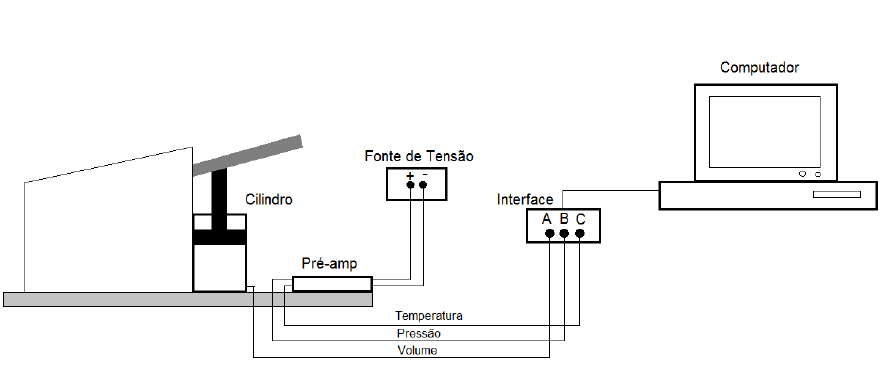
\includegraphics[width=260pt]{diagrama.png}
\begin{center}
\par\noindent {\scriptsize ({\bf Figura 1}: Diagrama da experiência)}
\end{center}
\end{center}

\begin{thebibliography}{9}

\bibitem{guia} Guia de objetivos do trabalho, Professor João Figueirinhas
\bibitem{apontamentos} Apontamentos das aulas teóricas
%\bibitem{site} Wikipedia, the free encyclopedia - Thermoelectric effect. [Online] Available from: \url{http://en.wikipedia.org/wiki/thermoelectric\_effect}
\end{thebibliography}

\vfill

\pagebreak

%\section{Anexos}
%\subsection*{\normalsize Material}
%\begin{itemize}
%\item Cenas
%\end{itemize}
%
%\subsection*{\normalsize Tabelas Completas de Resultados}
%\par Cenas

\end{multicols}

\end{document}

% FOTOGRAFIA
%\begin{center}
%\includegraphics[width=240pt]{NOME SEM EXTENSAO}
%\par\noindent {\scriptsize (Figura X: Descrição)}
%\end{center}

%NOVA SUBSECÇÃO
%\subsection*{\normalsize BLA BLA}

%TABELA
%\begin{center}
%\begin{tabular}{ x{1.5cm} ... }
%i & ... \tabularnewline
%\hline \hline
%1 & 4.15  & 0.15  & 2033 & -  \tabularnewline
%\end{tabular}
%\par\noindent {\scriptsize (Tabela X: Descrição)}
%\end{center}